\section{SSC Cashflow and NPV Models}
\label{sec:SSCNPV}

Imagine a portfolio of candidate projects, in which some of the decisions involve
either replacing an item now or postponing replacement and facing potentially higher
maintenance and replacement costs. We choose to assume that the item must either
be replaced now or in the future, and it is in this context we describe the
appropriate cashflow calculations. We then extend the discussion to allow the
planned replacement to occur in year 2 or 3, for example, rather than in year 1.

We assume that doing nothing is not an option, since the items under consideration
are of significant importance and, if not replaced in due course, would impose
an unacceptable risk to either safety or production.

Notation:

\begin{itemize}
	\item  \( p \) : probability of item failure for one year

	\item  \( C_{P} \) : cost of planned replacement

	\item  \( C_{U} \) : cost of unplanned replacement

	\item  \( C_{D} \) : cost of shutdown per day

	\item  \( D \) : number of days plant is off-line, if a shutdown occurs

	\item  \( N \) : number of years

	\item  \( R \) : discount rate
\end{itemize}


%\begin{comment}
We could incorporate additional parameters, such as weekly or monthly inspection costs,
fixed costs of shutdown in addition to the daily costs specified above, etc. That said,
the setting we describe allows us to illustrate key ideas in the cashflow
calculations for computing NPV.

We further assume that, if we do not replace the item, its failure time is a random
variable that follows a geometric distribution where the probability of failure in
one year is denoted by  \( p \) (i.e., the probability of survival over one year
is  \( 1-p \) ). Thus, if the plant faces a 20-year decision period, the probability
of survival up to year  \( t \) is  \(  \left( 1-p \right) ^{t} \), and the probability
of failing in year  \( t \)  is given by  \( p \left( 1-p \right) ^{t-1} \).

Here is pedantic but useful construct for thinking about the calculations that follow
is to visualize a {\it coin flip}  for each year, yielding a {\it fail}  or {\it no fail}
event for that given year. Immediately after the coin flip, appropriate costs are incurred.
In other words, this discrete view of time with Bernoulli trials is useful to simplify the
logic of the calculations, rather than viewing time as a continuum and teasing
out {\it what happened when} during a given year.

If the item is not replaced today (time  \( t=1 \) ), we can compute the expected
replacement cost in any year  \( t=1, 2, \ldots ,N-1 \)  as:\par

%\begin{comment}


\begin{equation}\label{npv_1}
\mbox{Expected Replacement Cost in Year } t=C_{U}p \left( 1-p \right) ^{t-1}
\end{equation}


Here, we incur this cost only if the coin flips yielded $``$no fail$"$  events in
years  \( t=1, 2, \ldots ,t-1 \), then a $``$fail$"$  event in year  \( t \)
(i.e., we incur the cost through the geometric random variable’s probability mass of having
the first failure in year  \( t \), which is given by  \( p \left( 1-p \right) ^{t-1} \)).

Since we assume the item must be replaced in year  \( N \)  if it has not already failed,
the expected replacement cost does \textit{not} depend on the result of a coin flip
in year  \( N \), in the same way that replacement in year 1 precludes dependence on
the year 1 coin flip. Rather, we incur this cost with certainty in year  \( N \),
as long as the item had not failed in previous years
\(  t=1, 2, \ldots ,N-1 \); In other words, the expected cost is given by:\par

%\begin{comment}

\begin{equation}\label{npv_2}
\mbox{Expected Replacement Cost in Year }N=C_{P} \left( 1-p \right) ^{N-1}
\end{equation}

where the planned replacement cost is used.

In order to illustrate the computation of the cash flows, we further assume that,
if the item is not replaced now, the plant faces a loss of revenue due to a shutdown
at a cost of  \( C_{D} \)  per day. In this case, the expected downtime cost incurred in
year  \( t=1, 2, \ldots ,N-1 \)  is given by:\par

\begin{equation}\label{npv_3}
\mbox{Expected Downtime Cost in Year }t=DC_{D}p \left( 1-p \right) ^{t-1}.
\end{equation}

Again, we assume that the planned replacement in year  \( t=N \)  precludes dependence
on the coin flip and therefore also precludes incurring any downtime cost in that year,
though we acknowledge other assumptions are possible. Thus, for practical purposes,
there is no coin flip in year  \( N. \)

More generally, if the item is not replaced now, the plant will face the possibility
of increased costs due to reliability issues. Such costs include increased
inspection costs, downtime costs for a week-long shutdown, lost revenue from a 6-hour
shutdown, costs associated with the emergency replacement of an item, etc. We can express
the above costs in the following functional form:
\( Re \_ Cost \left( p,t,C_{1},C_{2, \cdots , }C_{M} \right)  \),
where  \( C_{1},C_{2, \cdots, }C_{M} \)  are costs relevant for the considered item, and,
in general,  \( p \)  could be a vector that incorporates multiple types of shutdown. In
our case, the expected downtime cost in year  \( t=1, 2, \ldots ,N \)  is given by a function:
\( Re \_ Cost \left( p,t,C_{P},C_{U},C_{D},D,N \right)  \) , with just a scalar value for  \( p \).

There are two relevant time-series of cash flows: one for replacing the item now and
another for replacing it later, either at failure or at the horizon year  \( N \).
First, consider replacing the item today; in this case, we simply incur the cost of
planned replacement at time  \( t=1 \) (i.e., we incur cost  \( C_{P} \).)

The second time-series of cash flows is for replacing the item in the future.
In this case, for every year  \( t \), we have the expected replacement cost
and downtime cost. So, for any year  \( t=1, 2, \ldots ,N-1 \), the cash
flows will be computed as:\par

\begin{equation}\label{npv_4}
\mbox{Cash Flow Replaced in Year }t= - \left[  \left( C_{U}+DC_{D} \right)  p \left( 1-p \right) ^{t-1} \right]
\end{equation}


and for the final year as:\par

\begin{equation}\label{npv_5}
\mbox{Cash Flow Replaced in Year }N= - \left[ C_{P} \left( 1-p \right) ^{N-1} \right] .
\end{equation}


Note the minus sign in front of the cash flows because all of them are costs
(i.e., cash outflows). The timelines of the two options are illustrated as follows: \par



%%%%%%%%%%%%%%%%%%%% Figure/Image No: 1 starts here %%%%%%%%%%%%%%%%%%%%

\begin{figure}
    \centering
    \centerline{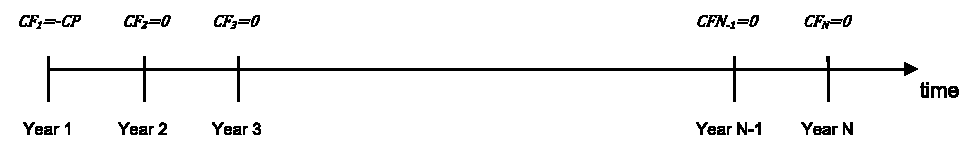
\includegraphics[scale=1]{image1.pdf}}
    \caption{Graphical representation of option 1: replace now.}
    \label{fig:_Graphical_representation_of_option_1_replace_now}
\end{figure}

%%%%%%%%%%%%%%%%%%%% Figure/Image No: 1 Ends here %%%%%%%%%%%%%%%%%%%%


%%%%%%%%%%%%%%%%%%%% Figure/Image No: 2 starts here %%%%%%%%%%%%%%%%%%%%

\begin{figure}
    \centering
    \centerline{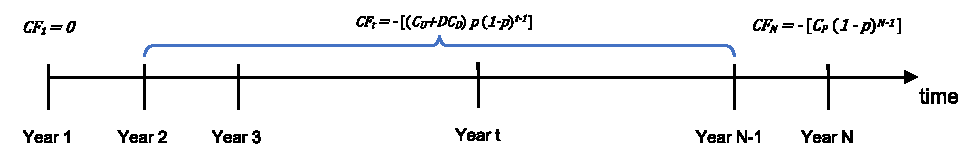
\includegraphics[scale=1]{image2.pdf}}
    \caption{Graphical representation of option 2: replace later.}
    \label{fig:_Graphical_representation_of_option_1_replace_later}
\end{figure}

%%%%%%%%%%%%%%%%%%%% Figure/Image No: 2 Ends here %%%%%%%%%%%%%%%%%%%%


The NPV of option 1 is: \par

\begin{equation}\label{npv_6}
\mbox{NPV option 1}= -C_{P}
\end{equation}

The NPV of option 2 is:\par

\begin{equation}\label{npv_7}
\mbox{NPV option }2= - \left[  \sum _{t=1}^{N-1}\frac{ \left( C_{U}+DC_{D} \right) p \left( 1-p \right) ^{t-1}}{ \left( 1+R \right) ^{t-1}}+\frac{C_{P} \left( 1-p \right) ^{N-1}}{ \left( 1+R \right) ^{N-1}} \right]
\end{equation}


We can compare these options in two ways. The first is to simply compute the
NPV as the difference between the NPV of option 1 and that of option 2 (i.e.,
\( \mbox{NPV}=\mbox{NPV option }1-\mbox{NPV option }2 \)). The resulting equation is:\par

\begin{equation}\label{npv_7}
\mbox{NPV}= -C_{P}+ \left[  \sum _{t=1}^{N-1}\frac{ \left( C_{U}+DC_{D} \right) p \left( 1-p \right) ^{t-1}}{ \left( 1+R \right) ^{t-1}}+\frac{C_{P} \left( 1-p \right) ^{N-1}}{ \left( 1+R \right) ^{N-1}} \right]
\end{equation}


If the project in question is the only one under consideration, and if  \( \text{NPV} \)  $>$ 0,
the decision is to replace the item today; otherwise, we replace it later.
%As we discuss in detail in Section 6, we\ employ an optimization model when multiple projects are considered simultaneously, and we need to stay within annual budgets in terms of, for example, capital costs.  \par

We now extend the above logic to the planned replacement occurring in year \( ~T_{0} \).
We had assumed  \( ~T_{0}=1 \), but now we allow for
delaying this planned replacement to a later year, albeit at the risk of incurring
a failure prior to  \( ~T_{0} \), along with associated unplanned\ replacement
and downtime costs.  If the planned replacement happens at time  \( T_{0} \), the
corresponding time-series of cash flows will become as follows: one for replacing the item
either at failure before  \( T_{0} \)  or at  \( T_{0} \),
and another for replacing it later, either at failure or at the horizon year  \( N \).\par

The first time-series of cash flows is for replacing the item at  \( T_{0} \).
In this case, for every year  \( t=1, 2, \ldots, T_{0}-1 \), we have the expected
replacement cost and downtime cost. So, for any year  \( 1, 2,\ldots, T_{0}-1 \),
the cash flows will be computed as:\par

\begin{equation}\label{npv_8}
\mbox{Cash Flow Replaced in Year }t= - \left[  \left( C_{U}+DC_{D} \right)  p \left( 1-p \right) ^{t-1} \right]
\end{equation}

for  \( t=T_{0} \)  the expected cash flow is:\par

\begin{equation}\label{npv_9}
\text{Cash Flow Replaced in Year }T_{0}= - \left[ C_{P} \left( 1-p \right) ^{T_{0}-1} \right]
\end{equation}

The timeline of this option is illustrated as follows: \par


%%%%%%%%%%%%%%%%%%%% Figure/Image No: 3 starts here %%%%%%%%%%%%%%%%%%%%

\begin{figure}
    \centering
    \centerline{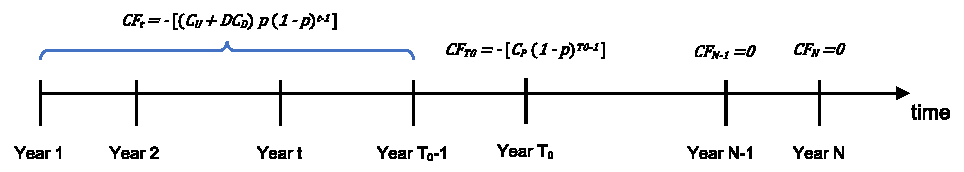
\includegraphics[scale=1]{image3.pdf}}
    \caption{Graphical representation of option 1: planned replacement at $T_0$.}
    \label{fig:_Graphical_representation_of_option_1_planned_replacement_at_}
\end{figure}

%%%%%%%%%%%%%%%%%%%% Figure/Image No: 3 Ends here %%%%%%%%%%%%%%%%%%%%

\begin{equation}\label{npv_10}
\mbox{NPV option }1= - \left[  \sum _{t=1}^{T_{0}-1}\frac{ \left( C_{U}+DC_{D} \right) p \left( 1-p \right) ^{t-1}}{ \left( 1+R \right) ^{t-1}}+\frac{C_{P} \left( 1-p \right) ^{T_{0}-1}}{ \left( 1+R \right) ^{T_{0}-1}} \right]
\end{equation}

Note that, if  \( T_{0}=1 \),  then the first term yields zero, and the NPV of
option 1 reduces to that discussed above (i.e., it equals  \( -C_{P} \).)\par

The second time-series of cash flow is for attempting to delay replacement of
the item to time  \( N \), and incurring the risk of unplanned replacement
and downtime in the meantime. It is the same as we calculated before. \par

\begin{equation}\label{npv_11}
\mbox{NPV option }2= - \left[  \sum _{t=1}^{N-1}\frac{ \left( C_{U}+DC_{D} \right) p \left( 1-p \right) ^{t-1}}{ \left( 1+R \right) ^{t-1}}+\frac{C_{P} \left( 1-p \right) ^{N-1}}{ \left( 1+R \right) ^{N-1}} \right]
\end{equation}

We can compute  \( \text{NPV} \)  as:\par

\begin{eqnarray}\label{npv_12}
\mbox{NPV}&=&\mbox{NPV Option }1-\mbox{NPV Option }2\\
&=& \left[  \sum _{t=T_{0}}^{N-1}\frac{ \left( C_{U}+DC_{D} \right) p \left( 1-p \right) ^{t-1}}{ \left( 1+R \right) ^{t-1}}+\frac{C_{P} \left( 1-p \right) ^{N-1}}{ \left( 1+R \right) ^{N-1}}-\frac{C_{P} \left( 1-p \right) ^{T_{0}-1}}{ \left( 1+R \right) ^{T_{0}-1}} \right]
\end{eqnarray}

A new RAVEN \textbf{External Model} with \xmlAttr{subType} \xmlString{LOGOS.IncrementalNPV}
was created to compute the NPV described above.

Example RAVEN Input \xmlNode{ExternalModel} XML:
\begin{lstlisting}[style=XML]
<ExternalModel name="rvi_model" subType="LOGOS.IncrementalNPV">
  <variables>fp,rvi_npv_a,rvi_npv_b</variables>
  <alias variable="rvi_p_failure" type="input">fp</alias>
  <Cp>19.82</Cp>
  <Cu>39.64</Cu>
  <fp>0.05</fp>
  <Cd>1.</Cd>
  <D>30</D>
  <options>
    <Td>1, 4</Td>
    <output>rvi_npv_a,rvi_npv_b</output>
  </options>
  <discountRate>0.03</discountRate>
  <startTime>2019</startTime>
  <lifetime>20</lifetime>
</ExternalModel>
\end{lstlisting}

In order to use this external model to compute NPV, \xmlString{LOGOS.IncrementalNPV}
should be always used for \xmlAttr{subType}. Except for the common nodes \xmlNode{variables}
and \xmlNode{alias}, this entity accepts the following sub-nodes:
\begin{itemize}
  \item \xmlNode{Cp}, \xmlDesc{float, required parameter}, specifies the cost of planned replacement.
  \item \xmlNode{Cu}, \xmlDesc{float, required parameter}, specifies the cost of unplanned replacement.
  \item \xmlNode{Cd}, \xmlDesc{float, required parameter}, specifies the cost of shutdown per day.
  \item \xmlNode{D}, \xmlDesc{integer, required parameter}, specifies the number of days
  plant is off-line, if a shutdown occurs.
  \item \xmlNode{fp}, \xmlDesc{float, required parameter}, specifies the probability
  of item failure over one year.
  \item \xmlNode{discountRate}, \xmlDesc{float, required parameter}, specifies the discount rate.
  \item \xmlNode{inflation}, \xmlDesc{float, optional parameter}, specifies the inflation rate.
  \default{0.0}
  \item \xmlNode{tax}, \xmlDesc{float, optional parameter}, specifies the tax rate.
  \default{0.0}
  \item \xmlNode{HardSavings}, \xmlDesc{float, optional parameter}, specifies the hard
  savings that would be added to the NPV calculation.
  \default{0.0}
  \item \xmlNode{count}, \xmlDesc{integer, optional parameter}, specifies the number
  of the same items/components that need to be replaced at the same time.
  \default{1.0}
  \item \xmlNode{startTime}, \xmlDesc{integer, required parameter}, specifies the
  start time of project.
  \item \xmlNode{lifetime}, \xmlDesc{integer, required parameter}, specifies the lifetime
  of the project.
  \item \xmlNode{options}, \xmlDesc{optional parameter}, specifies options to compute
  NPVs of planned replacements occurring in different years relative to the start time.
  \begin{itemize}
    \item \xmlNode{Td}, \xmlDesc{comma separated integers, required parameter},
    specifies the lengths of delaying the planned replacement.
    \item \xmlNode{output}, \xmlDesc{comma separated strings, required parameter},
    specifies the output variables corresponding to the different specified lengths of
    delays in \xmlNode{Td}. In order to communicate with RAVEN, these
    variables need to be listed under node \xmlNode{variables}.
    \nb These variables are defined by the user and would be used to store the
    calculated NPVs.
  \end{itemize}
\end{itemize}

The parameters \textbf{Cp, Cu, fp, Cd, inflation, and tax} can be sampled by RAVEN.
If the user specifies these parameters in the input XML \xmlNode{ExternalModel},
the values for these parameters will be replaced by the sampled values from RAVEN.

Example LOGOS Incremental NPV output CSV:
\begin{lstlisting}[language=python]
fp,rvi_npv_a,rvi_npv_b
...
\end{lstlisting}

\nb In order to compute the NPVs, the TEAL plugin is required.
Refer to ~\url{https://github.com/idaholab/raven/wiki/Plugins} for
details on how to access and install the plugins.

The whole calculation flow is depicted in Fig.~\ref{fig:LogosRAVEN}.

%%%%%%%%%%%%%%%%%%%% Figure/Image No: 4 starts here %%%%%%%%%%%%%%%%%%%%

\begin{figure}
    \centering
    \centerline{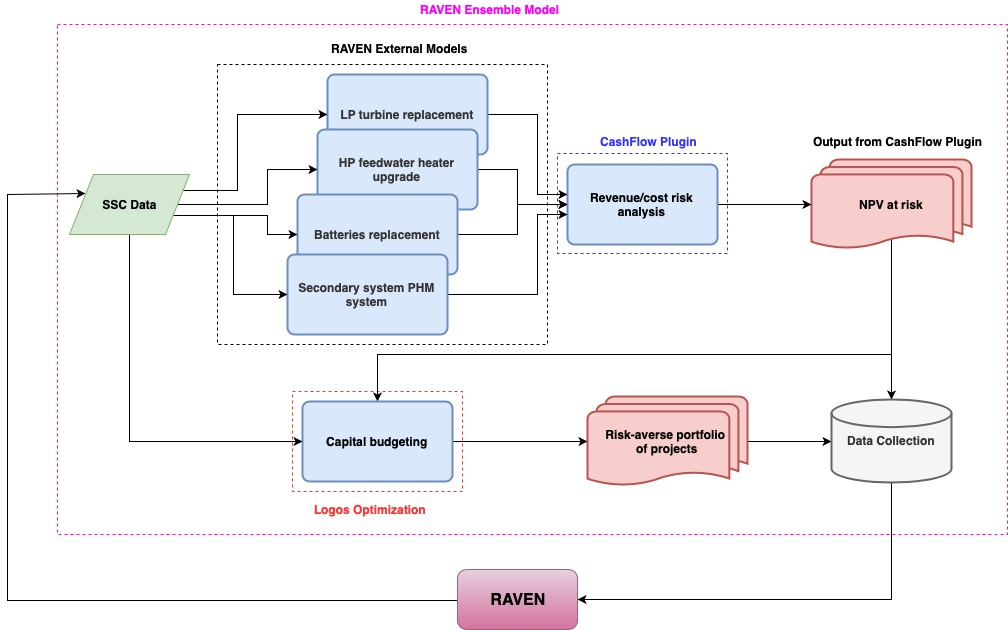
\includegraphics[scale=0.5]{image11.jpg}}
    \caption{Risk-informed capital budgeting via RAVEN and RAVEN plugins.}
    \label{fig:LogosRAVEN}
\end{figure}

%%%%%%%%%%%%%%%%%%%% Figure/Image No: 4 Ends here %%%%%%%%%%%%%%%%%%%%
